\documentclass[a4paper]{report}
\usepackage{graphicx}
\usepackage{float}
\usepackage{eso-pic}
\usepackage{hyperref}
\usepackage[italian]{babel}
\usepackage{booktabs}

\newcommand{\quotes}[1]{``#1''}
\newcommand\BackgroundPic{%
	\put(0,0){
		\parbox[b][\paperheight]{\paperwidth}{%
			\vfill
			\centering
			
\includegraphics[width=\paperwidth,height=\paperheight,%
			keepaspectratio]{its-cover.pdf}%
			\vfill
		}
	}
}
\hypersetup{
	colorlinks=true,
	linkcolor=blue,
	filecolor=magenta,
	urlcolor=blue,
	pdftitle={Report Finale \quotes{Laboratorio Integrato}},
	pdfpagemode=FullScreen,
}
\graphicspath{ {../ImmaginiReportFineProgetto/} }

\author{De lazzari, Dellera, Oglietti,\\
 Murta, Cafasso, Carrieri}
\title{Report Finale \quotes{Laboratorio Integrato}\\
\large Gruppo 6, Cloud Fiesta}
\date{\today}
\makeindex

\begin{document}
\AddToShipoutPicture*{\BackgroundPic}
\maketitle
\tableofcontents
\chapter{Introduzione}\label{introduzione}
	\section{Il Progetto}\label{il_progetto}
		Il qui presente report ha lo scopo di illustrare lo svolgimento del progetto a opera del gruppo \quotes{Cloud
		Fiesta}, il progetto e' stato commissionato dai docenti Blanchietti Andrea e Zimuel Enrico nell'ambito del corso
		\textit{\quotes{Laboratorio Integrato}}.
		
		Lo scopo del progetto e' quello di realizzare una piattaforma di \emph{e-commerce} per conto di un azienda che
		si occupa di commercio al dettaglio, il sistema deve essere \emph{scalabile} in maniera da poter limitare i
		costi a quanto strettamente necessrio e potersi mantenere aderente con le esigenze di crescita aziendale.
		Inoltre, e' essenziale che la piattaforma possa avere degli \emph{standard di sicurezza elevati}, come ben
		sappiamo, durante i recenti anni si e' verificata un impennata dei crimini legati alla \textit{Cybersecurity},
		con un particolare aumento durante la corrente pandemia da COVID-19, come illustrato
		\href{https://www.interpol.int/en/News-and-Events/News/2020/INTERPOL-report-shows-alarming-rate-of-cyberattacks-during-COVID-19}{dall'Interpol}.
		E' quindi fondamentale che un'applicazione che gestisce flussi di denaro sia quindi estremamente solida dal
		punto di vista della sicurezza informatica.  Una seconda sezione del progetto, prevede che ogni gruppo si occupi
		di eseguire dei \emph{penetration test} sul gruppo dall'\emph{ID} successivo. Questo per simulare l'ingaggio di
		un azienda esterna allo scopo di testare la sicurezza di un prodotto prima di rilasciarlo effettivamente sul
		mercato, uno step di decisiva importanza che permettera' ai componenti di ogni gruppo di sperimentare le proprie
		conoscenze di sicurezza informatica all'interno di una situazione altamente realistica.

		Vista la complessita' del progetto, e' stato scelto di realizzarlo tramite Team multidisciplinari, con
		componenti appartenenti ad due corsi afferenti agli indirizzi di \emph{Cloud Specialist} e \emph{ICT Security
		Specialist}.  All'interno di questi due corsi sono presenti le competenze tecniche atte a svolgere il progetto
		commissionato, coprendo sia l'area di sicurezza e di architettura della rete interna, che quella di utilizzo
		delle piattaforme cloud che permettono di assicurare la scalabilita' necessaria all'azienda.
	\section{Il Team}\label{il_team}
		Gli stutenti di entrambi i corsi sono stati divisi in sei differenti gruppi, composti da un totale di otto persone,
		il nostro gruppo, denominato \quotes{\emph{Cloud Fiesta}} e' composto dai seguenti studenti:
		\begin{itemize}
			\item \textbf{Cafasso Giovanni}
			\item \textbf{Carrieri Riccardo}
			\item \textbf{De Lazzari Riccardo}
			\item \textbf{Dellera Lorenzo}
			\item \textbf{Murta Alessio}
			\item \textbf{Oglietti Riccardo}
			\item \textbf{Zuccarella Andrea}
		\end{itemize}
		Suddivisi rispettivamente all'interno dei due corsi come da tabella:
		\begin{center}
			\begin{tabular}{c c}
				Cloud Specialist & ICT Security Specialist \\
				\midrule
				Cafasso Giovanni & De Lazzari Riccardo \\
				Carrieri Riccardo & Dellera Lorenzo \\
				Murta Alessio & Oglietti Riccardo \\
				Zuccarella Andrea & \\
			\end{tabular}
		\end{center}
		Come consigliato dai docenti, sono stati assegnati alcuni \emph{ruoli} in grado di aiutarci con l'organizzazione
		delle mansioni e in genere della gestione del progetto, in particolare abbiamo individuato il ruolo di
		\emph{Team Leader} e di e di \emph{Co-Team Leader}, essi sono stati rispettivamente assegnati a \emph{Oglietti
		Riccardo} e \emph{Murta Alessio}. Abbiamo optato per assegnare queste due cariche ripartendole tra i due
		differenti corsi che compongono il gruppo in maniera da manternere un buon livello di equita' e rappresentanza
		per entrambe le anime del team.

\chapter{Strumenti tecnico-organizzativi}
	\section{GANTT e cronoprogramma}\label{gantt_e_cronoprogramma}
		Innanzitutto parlando di strumenti tecnico-organizzativi non e' possibile iniziare senza descrivere il
		\emph{GANTT}.  Strumento principe per l'organizzazione delle tempistiche, si tratta di una tabella a doppia
		entrata che permette di assegnare alcuni \emph{task} ritenuti fondamentali a un membro e un momento nel quale
		realizzarlo.

		Ecco una lista riassuntiva dei processi e degli \emph{step} fondamentali che abbiamo individuato al fine della
		realizzazione ottimale del progetto, divisi in base al corso di afferenza dei destinatari:
		\begin{itemize}
			\item \begin{enumerate}
					\item Parsing file CSV
					\item Definizione struttura di rete
					\item Deploy infrastruttura
					\item Test di sicurezza
					\item Modfica struttura in base alle falle trovate
					\item Deploy infrastruttura finale
					\item Implementazione certificato SSL
					\item Stesura report
					\item Stesura presentazione Powerpoint
				\end{enumerate}
			\item \begin{enumerate}
					\item Brainstorming
					\item Test locali nopCommerce
					\item Revisione manuale catalog.csv
					\item Scelta infrastruttura cloud
					\item Containerazziazione su distribuzione GNU/Linux
					\item Personalizzazione docker image nopCommerce
					\item Caricamento su Cloud Provider
					\item Gestione e implementazione metodo di pagamento
					\item Calcolo dei prezzi e stesura report economico
					\item Gestione permessi utenti in Azure
				\end{enumerate}
		\end{itemize}
	\section{Strumenti di comunicazione}\label{strumenti di comunicazione}
		Durante il primo incontro uno dei principali punti che e' stato chiarito e' quello della \emph{comunicazione}.
		E' infatti essenziale che in un gruppo di lavoro sia possibile gestire la comunicazione in maniera piu'
		efficente e inclusiva possibile, senza quindi escludere membri o affidarsi a piattaforme troppo lente o non
		organizzate.
		
		La scelta e' quindi ricaduta sulla piattaforma di messaggistica istantanea \emph{Telegram}, grazie alla
		puntualita' delle opzioni di gestione di una \emph{chat} di gruppo e' possibile \emph{fissare} messaggi, creare
		sondaggi e inviare file di grandi dimensioni. Grazie a recenti aggiornamenti e' inoltre possibile effettuare
		videochiamate e condividere eventualmente il proprio desktop, una feature essenziale nel campo del lavoro
		collaborativo.
	\section{Organizzazione codice}\label{organizzazione codice}
		Data la forte componente di scrittura software presente all'interno del progetto, si e' propenso per l'utlizzo
		di una piattaforma di sviluppo collaborativo, in maniera da organizzare la stesura del codice nella maniera piu'
		semplice ed esaustiva possibile. In particolare ci siamo affidati al software \emph{GIT} a opera di \emph{Linus
		Torvalds}, creando un organizzazione sulla popolare piattaforma di proprieta' \emph{Microsoft}, \emph{GitHub}.

		Sulla piattaforma ci siamo quindi premurati di creare immediatamente tre \emph{repository} atti a contenere il
		lavoro prodotto dal gruppo, in particolare essi sono:
		\begin{enumerate}
			\item \texttt{Random\_Script}\label{item:Script}
			\item \texttt{Report}\label{item:Report}
			\item \texttt{Report\_Economy}\label{item:ReportE}
		\end{enumerate}

		Il repository numero \ref{item:Script}{, \emph{Random\_Script}} e' atto al contenimento di una serie di
		programmi di piccola entita', come il \emph{parser} che si e' occupato di scaricare le immagini dei prodotti da
		aggiungere successivamente al database dello store, o il \emph{docker-compose.yml} che servira' per effettuare l'operazione di \emph{deploy} sull'infrastruttura in ambiente di produzione.

		Per quanto riguarda \emph{Report}, ossia il numero \ref{item:Report}, si tratta dello spazio atto alla creazione
		del report finale, esso e' stato redatto tramite l'utilizzo del linguaggio \LaTeX{}, argomento che sara'
		affrontato in dettaglio in seguito.

		Infine, il \emph{repository} \ref{item:ReportE}, nominato come \emph{Report\_Economy}, e' atto ad accogliere i
		documenti e gli appunti che permetteranno la stesura di un preventivo attendibile dell'implementazione, come
		richiesto dai requisiti del progetto.
	\section{Strumenti di scrittura}\label{strumenti_di_scrittura}
		Come accennato durante la precedente sezione, lo strumento principe che e' stato impiegato per la redazione
		della relazione di progetto e' stato li linguaggio \LaTeX{}. Si tratta di un linguaggio in grado di produrre un
		testo correttamente formattato a partire da semicodice, in questo modo viene automatizzata la gestione di alcune
		importanti caratteristiche del documento finale, come per esempio le immagini, spesso punto di debolezza dei
		comuni software di videoscrittura.
\chapter{Componenti e architettura}\label{componenti_e_architettura}
	\section{In generale}\label{in_generale}
		\subsection{Provider servizi cloud}\label{provider_servizi_cloud}
			Parlando di \emph{provider} di servizi \emph{cloud}, e' doveroso premettere come l'infrastruttura e' stata
			concepita allo scopo di essere completamente indipendente da un particolare marchio o servizio esterno. Essa
			e' stata pensata in maniera da essere facilmente implementata su una varita' di fornitori di servizi
			\emph{cloud} differenti, in maniera da poter agilmente scegliere quello piu' conveniente per l'azienda
			committente in maniera indipendente dalla piattaforma. Fatto salvo cio', l'intera descrizione del progetto
			e' basata su quanto sviluppato sulla piattaforma \emph{Microsoft Azure} di cui di seguito, al fine di poter
			mantenere la descrizione il piu' semplice e lineare possibile.
		\subsection{Microsoft Azure}\label{microsoft_azure}
			Per descrivere l'architettura ideata riteniamo importante descrivere il \emph{provider} principale sul quale
			e' stato deciso di fare affidamento. La scelta e' ricaduta sullo strumento \quotes{\emph{Microsoft Azure}}:
			si tratta di un servizio di \emph{Cloud Computing} offerto da \emph{Microsoft} che, come il resto dei
			\emph{provider} sul mercato nel medesimo campo, offre servizi di \emph{Infrastructure as a Service},
			\emph{Platform as a Service} e \emph{Software as a Service}.
			In particolare, la scelta e' ricaduta su questo servizio per via della semplice integrazione con gli account
			\emph{Microsoft}, che ha permesso una gestione dei permessi di accesso alle macchina granulare e semplice da
			gestire.
			Inoltre, come molti dei suoi piu' diretti concorrenti, \emph{Microsoft} offre un bonus gratuito di \$100 da
			spendere sulla piattaforma per ogni persona che vi si registri come studente. Cio', in concomitanza con
			i prezzi in linea con il mercato ha permesso sperimentazioni senza il rischio di dilapidare denaro.
		\subsection{nopCommerce}\label{nopcommerce}
			Durante la nostra ricerca di una soluzione che ci permettesse di creare uno \emph{store online} ci siamo
			imbattuti in \emph{nopCommerce}, una tecnologia a opera di \emph{nopSolutions}. Si tratta di una soluzione
			\href{https://github.com/nopSolutions/nopCommerce/blob/develop/LICENSE.md}{\emph{libre}} e
			\emph{open source} che permette la creazione di \emph{store online} mantanendo una discreta
			semplicita' di utilizzo, nonche una facile integrazione in ogni sistema grazie alla possibilita' di essere
			installato all'interno di un \emph{contatiner Docker}.

			Nato nel 2008, sviluppo e supporto non si sono mai interrotti, l'ampia \emph{community} che lo mantiene
			e lo sviluppa permette inoltre una facile risoluzione di eventuali problemi grazie all'ampia
			\href{https://docs.nopcommerce.com/en/developer/index.html?utm\_source=github&utm\_medium=referral&utm\_campaign=documentation&utm\_content=text}{documentazione}
			prodotta nel corso degli anni. Questo prodotto abbraccia le moderne tecnologie in ambito di sviluppo web e
			di sicurezza grazie al massiccio utilizzo di \emph{ASP.NET Core 5} e all'utilizzo come database predefinito
			di \emph{MySQL} fino alle ultime versioni stabili. 
	\newpage
	\section{Architettura di rete}\label{architettura_di_rete}%Inserire grafichetto della struttura
		L'architettura di rete scelta e' basata sull'utilizzo di una singola macchina virtuale in \emph{cloud} sulla
		sopracitata piattaforma \emph{MS Azure}.

		La macchina virtuale monta un sistema operativo \emph{GNU/Linux Ubuntu Server 20.04 LTS}, e ha le seguenti
		caratteristiche:
		\begin{center}
			\begin{tabular}{c c}
				Informazione & Metrica \\
				\midrule
				Tipologia & Standard\_D2s\_v3 \\
				CPU & 2 \\
				RAM & 8 GB \\
				Disco & 30 GB SSD Premium con ridondanza locale \\
				Sicurezza & Standard \\
			\end{tabular}
		\end{center}

		Al suo interno sono poi presenti alcuni elementi aggiuntivi, che compongono la vera e propria infrastruttura.

		Innanzitutto e' presente \emph{Docker}, si tratta del \emph{runtime} piu' diffuso per \emph{container} diffuso
		sul mercato. I \emph{container} sono \quotes{entita'} che al loro interno contengono un ambiente minimale con
		tutte le componenti necessarie a un applicativo per svolgere il suo funzionamento, comprese tutte le dipendenze
		di ognuna delle sue parti. Questa entita' si interfaccia poi con il \emph{Docker Engine}, un software che si
		occupa di tradurre le richieste del container in chiamate al sistema operativo sottostante, in questo caso una
		distribuzione di \emph{Ubuntu GNU/Linux}.

		Da sottolineare poi la fondamentale presenza di \emph{SSH}\label{SSH}. Si tratta dell'implementazione
		dell'omonimo protocollo di connessione remota per sistemi operativi \emph{UNIX like}. Esso permette di
		effettuare una connessione remota con una macchina tramite una coppia di credenziali oppure attraverso una chiave
		\emph{RSA}, criptando il traffico in maniera da mantenere la riservatezza della comunicazione.

		Infine, gli ultimi due applicativi che e' opportuno segnalare come parti fondamentali della topografia di rete
		sono \emph{Uncomplicated FireWall} e \emph{Fail2Ban}. Il primo, come intuibile dal nome, e' un \emph{Firewall}
		atto a limitare le connessioni non autorizzate verso la macchina per il quale e' configurato. In particolare,
		questo firewall e' in realta' un \emph{frontend} semplificato per \emph{IP Tables}, probabilmente il piu'
		utilizzato firewall in ambiente \emph{GNU/Linux}.
		Anche \emph{Fail2Ban} si occupa di una funzione simile, in quanto la sua funzione prinicpale all'interno dell'
		architettura proposta e' quella di regolamentare e limitare l'accesso alle connessioni \emph{SSH} per i soggetti
		non autorizzati.

		In figura \ref{fig:architettura_di_rete} una rappresentazione grafica di quanto illustrato.

	\section{Organizzazione container}\label{organizzazione_container}
		Come accennato durante il precedente paragrafo, la nostra architettura e' organizzata tramite l'utilizzo di
		\emph{container}. Questa metodologia di  \emph{deploy} e' stata scelta perche offre numerosi vantaggi rispetto
		alla piu' \quotes{classica} architettura basata sull'utlizzo di macchine virtuali dedicate. In particolare, una
		macchina e' in grado di gestire diversi \emph{container}, ottimizzando al meglio le risorse
		\emph{hardware} a disposizione. Inoltre, il parziale isolamento di un \emph{container} rispetto alla macchina
		\emph{host} rende l'infrastruttura piu' sicura, in quanto compromettere un singolo applicativo non mette a
		rischio il resto dell'infrastruttura o degli altri servizi che condividono le medesime risorse.
		Infine e' importante sottolineare che, grazie all'utilizzo di \emph{Docker Compose},uno strumento per la 
		definizione e l'esecuzione di applicazioni \emph{Docker} multi-contenitore, possiamo utilizzare un singolo comando per
		creare e avviare tutti i container definiti nel file yaml. Non solo, ci permette di definire e collegare in una
		rete logica i \emph{container}, che interagiranno tra loro come fosserò macchine fisiche.
		Per implementare la nostra infrastruttura, abbiamo deciso di utilizzare i seguenti \emph{container}:
		\begin{itemize}
			\item nopCommerce
			\item MySQL
		\end{itemize}
		Il primo denominato come \emph{nopCommerce} contiene l'effettiva struttura dello \emph{store online}, compreso
		%%%%%%%%%%%%%%%%%%%%%%%%%%%%%%%%%%%%%%%%%%%%%%%ocio alla porta%%%%%%%%%%%%%%%%%%%%%%%%%%%%%%%%%%%%%%%%%%%%%%%%%%
		di tutte le componenti atte a pubblicare le pagine \emph{web} sulla porta \texttt{8080}.
		
		Il secondo \emph{contaier} invece, contiene un database \emph{MySQL} che si occupera' di contenere tutte le
		informazioni riguardanti i prodotti, i clienti, gli acquisti e molto altro.
		
		Ecco alcuni dei campi presenti all'interno del \emph{database}
		\begin{enumerate}
			\item ProductId
			\item ProductType
			\item Name
			\item FullDescription
			\item Vendor
		\end{enumerate}

		I \emph{container} sono configurati in maneira da utilizzare due porte per la comunicazione: la porta
		\texttt{80} e la porta \texttt{3306}. Rispettivamente usate per permettere al \emph{container} contenente
		\emph{nopCommerce} di essere esposto verso internet, e sempre al medesimo di effettuare le comunicazioni con il
		database \emph{MySQL}.

		\begin{figure}[H]
			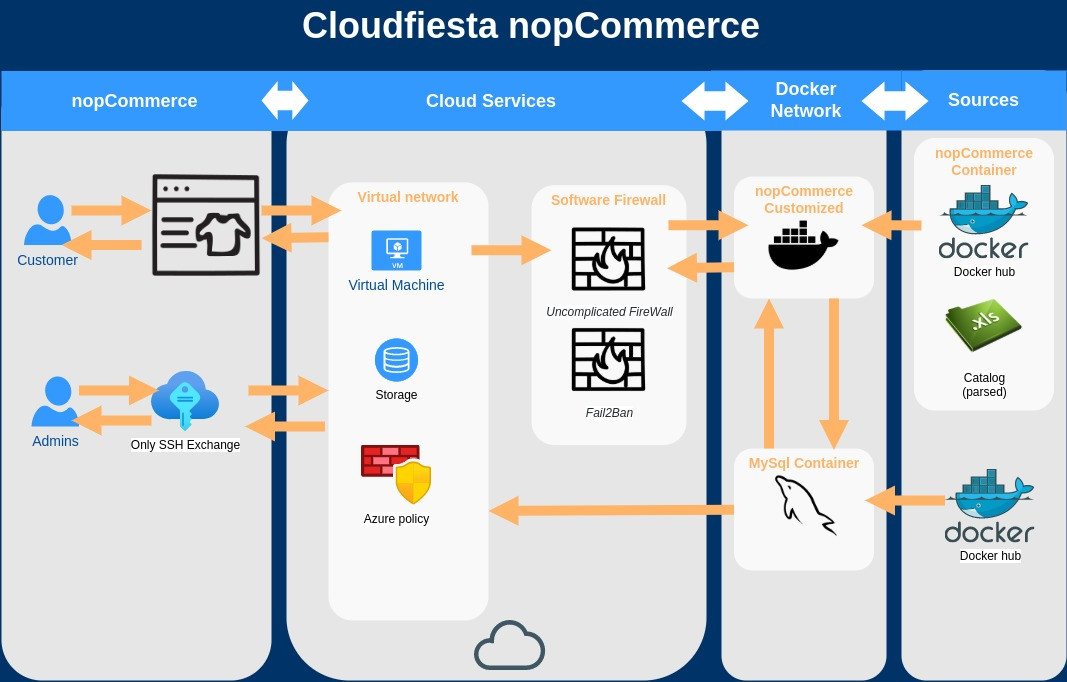
\includegraphics[scale=0.3]{DiagrammaDiRete.jpg}\label{fig:architettura_di_rete}
			\caption{Infrastruttura di rete}
		\end{figure}
 

\chapter{Processo di implementazione}\label{processo_di_implementazione}
	Per gestire al meglio le tempistiche e la messa a terra del progetto abbiamo strutturato un processo diviso in fasi,
	esse ci hanno permesso di poter controllare lo stato di avanzamento dei lavori e modificare i programmi e il carico
	di lavoro in maniera coerente. In particolare possiamo individuare tre principali fasi, elencate di seguito;
	\begin{enumerate}
		\item Brainstorming e ricerca
		\item Prototipazione e scripting
		\item Implementazione locale
		\item Implementazione remota
		\item Test di sicurezza
	\end{enumerate}
	Ognuna di queste fasi del lavoro ha occupato un diverso ruolo e ha necessitato sforzi di natura diversa, ecco dunque
	presentata una breve sintesi di quanto accaduto in ognuna di esse.
	\section{Brainstorming e ricerca}\label{brainstorming_e_ricerca}
		Durante la prima parte del progetto, il gruppo si e' dedicato all'individuazione degli strumenti precedentemente
		citati atti all'implementazione di quanto richiesto. Questo iniziale sforzo e' stato portato avanti
		contemporanemente da tutti i membri del gruppo, mentre i membri afferenti al corso di \emph{Cloud Specialist} si
		sono occupati di effettuare le necessarie ricerce per quanto riguarda il provider di servizi, i membri di
		\emph{ICT Security Specialist} si sono occupati di iniziare a definire acluni strumenti atti alla gestione della
		rete.
		Durante questa fase iniziale, sono stati inoltre individuati lo strumento atto alla creazione dello \emph{store
		online}, la relativa gesione del \emph{database} e tutti gli strumenti di comunicazione, organizzazione e
		videoscrittura.
	\section{Prototipazione e scripting}\label{prototipazione_e_scripting}
		La fase successiva si e' rivalta essere molto piu' pratica di quella appena svolta, in quanto il gruppo si e'
		trovato a dover iniziare a risolvere alcuni problemi pratici, come il \emph{parsing} del file \emph{csv}
		contenente i dati atti a popolare il \emph{database} e l'utilizzo di \emph{nopCommerce}.

		La necessita' di agire sul file originale contenente i dati iniziali per popolare il \emph{database} e' nata
		dalla scelta operata dal team di sicurezza di mantenere una copia delle immagini localmente alla macchina in
		maniera da ridurre il perimetro di vulnerabilita' dell'infrastruttura. Senza questo passaggio, il
		\emph{database} conterrebbe collegamenti a risorse esterne, i quali potrebbero essere sfruttati da attori
		terzi per ottenere accesso o controllo a parti dell'infrasturttura.

		E' quindi stato prodotto uno \emph{script} tramite  il linguaggio \emph{bash} che, partendo da una trascrizione
		in formato testuale del file originale, possa ottenere le immagini relative ai prodotti conservandone il
		corretto ordine e il riferimento al prodotto. Questo compito e' stato reso piu' difficile da alcuni problemi di
		formattazione conentuti all'interno del file originale. Come prima azione, lo \emph{script} si occupa di
		controllare che tutti gli \emph{URL} siano validi e non nulli, dopodiche procede con l'effettivo scaricamento e
		indicizzazione delle immagini, in figura \ref{fig:script} un'estratto dal sopracitato script.

		\begin{figure}[H]
			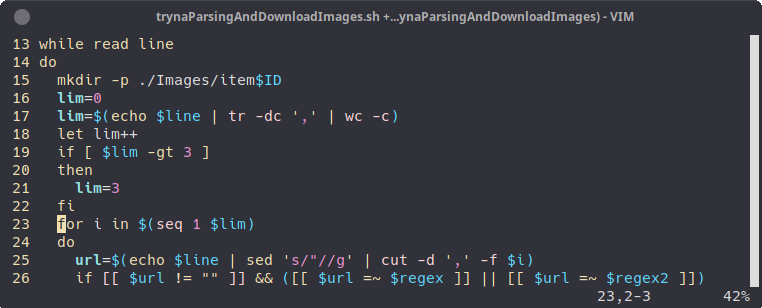
\includegraphics[width=\textwidth]{Script.png}\label{fig:script}
			\caption \\Script atto al \emph{download} delle immagini.
		\end{figure}

		Durante questa fase sono state esplorate le varie opzioni per l'implementazione di \emph{nopCommerce},
		considerando quale sistema operativo e strategia di \emph{deploy} scegliere tra le diverse disponibli.
	\section{Implementazione locale}\label{implementazione_locale}
		La fase logicamente successiva ha quindi previsto l'implementazione per intero dello \emph{store} localmente,
		in maniera da poter evidenziare eventuali criticita' e difficolta' di messa in produzione. In particolare
		l'utilizzo del \emph{database} ha inizialmente creato alcune difficolta', al fine di condurre test e
		sperimentazioni e' stato scelto di usare \emph{MySQL} tramite il gruppo di \emph{software} orientato alla
		programmazione \emph{WEB} \emph{XAMPP}. Si tratta di uno \emph{stack} di \emph{software} comunemente usato
		all'interno della programmazione \emph{WEB}, l'acronimo simboleggia i \emph{software} conenuti al suo interno,
		ossia:
		\begin{center}
			\begin{tabular}{c c}
				X & Cross-Plattform \\
				A & Apache WEB-server \\
				M & MySQL \\
				P & PhP \\
				P & Pearl \\
			\end{tabular}
		\end{center}
		In particolare, le difficolta' sono state riscontrate nell'importazione del \emph{database}: \emph{nopCommerce}
		sfrutta una serie di parametri non presenti all'interno del file originariamente fornitoci, e' quindi stata
		necessaria un'operazione di modifica per adattare il file iniziale alle esigenze della piattaforma da noi
		scelta.
		Prima di giungere a questa soluzione, sono state riscontrate diverse anomalie, per esempio l'impossibilita' di
		visualizzare i prodotti ottenuti, o di aggiungerli al \quotes{carrello} per terminare l'acquisto.
		Il problema e' stato finalmente risolto tramite l'esportazione della tabella \emph{products} tramite
		l'interfaccia alla piattaforma per comprenderne al meglio la struttura, e poter di conseguenza strutturare il
		file \emph{CSV} in maniera consona.
		Una volta utlimata un implementazione completamente funzionante della piattaforma di \emph{e-commerce}
		localmente, e' iniziata la sperimentazione remota, descritta in maniera piu' completa di seguito.
	 \section{Implementazione remota}\label{implementazione_remota}
		Durante la fase di implementazione remota, lo scopo del gruppo e' stato quello di ottenere un infrastruttura
		funzionante e completa, compresa di dati e grossolane misure di sicurezza, da poter poi raffinare fino
		all'ottenimento del risultato finale.

		Il processo e' partito dalla creazione di una macchina virtuale con le caratteristiche descritte nella sezione
		\ref{architettura_di_rete}, il gruppo si e' poi cimentato nella gestione degli accessi alla sopracitata
		macchina, dapprima tentando un approccio basato sulle organizzazioni e i gruppi offerti nell'ambito della
		piattaforma \emph{Microsoft Azure}, terminando poi con il piu' intuitivo sistema offerto nativamente dal sistema
		operativo scelto basato sul protocollo \emph{SSH} descritto nella sezione \ref{SSH}.
		Il primo approccio ha presentato diverse difficolta' legate inizialmente all'assegnazione di tutti i componenti
		del gruppo a una singola untia' organizzativa, seguite poi da difficolta' di assegnazione dei necessari permessi
		per poter ottenere visibilita' sulla macchina che avrebbe ospitato l'infrastruttura e infine dell'asegnazione di
		chiavi di accesso univoche a tutti i membri. E' stato quindi scelto di lasciare la creazione della macchina e di
		un primo account con privilegi amministrativi a un membro, il quale ha poi condiviso le credenziali necessarie
		alla connessione remota tramite comunicazione criptata. Da questo primo account amministrativo e' stato poi
		possibile impostare profili personali per ognuno dei membri del gruppo, dotando ognuno dei minimi privilegi
		necessari allo svolgimento della sua funzione secondo il principio \quotes{\emph{Least Privilege}}. In figura
		\ref{fig:utenti_e_gruppi} sono illustrati i gruppi di appartenenza di ciascun utente.

		\begin{figure}[H]
			%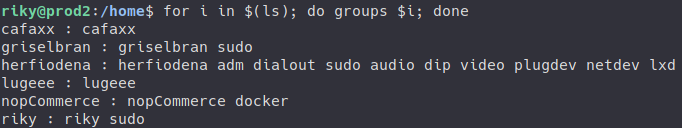
\includegraphics[scale=0.5]{UtentiEGruppi.png}\label{fig:utenti_e_gruppi}
			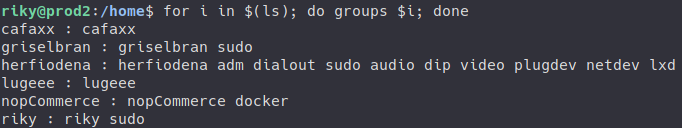
\includegraphics[width=\textwidth]{UtentiEGruppi.png}\label{fig:utenti_e_gruppi}
			\caption \\Gruppi di afferenza per ogni utente
		\end{figure}

		Ognuno dei profili utente creati e' dotato di una coppia di chiavi \emph{RSA} generata tramite il comando
		\texttt{ssh-keygen -b 4048}, che, in congiunzione con le coppie di chiavi delle macchine dei rispettivi membri
		del gruppo ha permesso di impostare un accesso ai profili utenti tramite chiave univoca. 
		Grazie a questi scambi di chiavi, e' stato succcessivamente possibile disabilitare l'accesso via \emph{password}
		a tutti gli utenti, rinforzando notevolmente la sicurezza della macchina e dell'infrastruttura. E' poi stato
		creato un utente denominato \emph{nopCommerce} abilitato ad utilizzare solamente i comandi indispensabili alla
		gestione dei container contenenti la piattaforma e il relativo \emph{database}. Questo account e' inoltre privo
		di chiavi e inibito dallo stabilire connessioni \emph{SSH} in entrata o in uscita tramite l'utilizzo di
		\emph{policy}, in maniera da renderlo accessibile solamente da un utente all'interno della macchina tramite il
		comando \texttt{su}, protetto da una \emph{password} notevolmente robusta. Una volta terminata la messa in rete
		della piattaforma di \emph{e-commerce} l'utente \emph{nopCommerce} e' stato ulteriormente limitato tramite
		l'ipostazione della \emph{shell} \texttt{/sbin/nologin} come interfaccia predefinita dell'utente, in questa
		maniera, anche se in possesso delle credenziali di accesso di un utente, e' comunque impossibile effettuare il
		\emph{login} all'\emph{account} \emph{nopCommerce} in quanto esso non ha un effettiva \emph{shell} interattiva
		con la quale interfacciarsi.
		Inoltre, sia tramite l'interfaccia di \emph{Microsoft Azure} sia tramite il \emph{firewall} implementato, sono
		state definite alcune \emph{policy} atte a limitare l'accesso all'infrastruttura da parte di soggetti non
		autorizzati. In particolare le \emph{policy} sono state suddivise principalmente in due categorie: quelle legate
		alle connessioni \emph{SSH}, gestite da \emph{Fail2Ban} e \emph{UFW}; e quelle gestite dalla piattaforma
		\emph{Azure}, atte principalmente all'amministrazione delle connessioni verso la macchina virtuale e le sue
		porte.

		Grazie alla fase di produzione in locale, e' stato possibile definire una serie di passaggi per rendere piu'
		agile il \emph{deploy} dell'infrastruttura, partendo dall'immagine ufficiale di \emph{nopCommerce} disponibile
		su \emph{Docker Hub}, e' stato possibile costruirne una personalizzata, contenente direttamente le immagini
		afferenti ai prodotti presenti all'interno del cataglogo.  La nuova immagine è custodita in repository privato
		sulla piattaforma \emph{Docker Hub}, funzionale solo al nostro progetto.  Bastera' dunque lanciare il commando
		\texttt{docker-compose up}, per ottenere in pochi minuti l'intera infrastruttura, attiva e pronta per la
		produzione.  Questo espediente, insime a due file di configurazione in formato execel, da la possibilita' di
		mettere in produzione la piattaforma \emph{ e-commerce} in pochi minuti, in maniera totalmente indipedente dal
		\emph{provider} di servizi \emph{cloud} utilizzato.

		L'ultima fase della \quotes{sperimentazione} sulla macchina di prova si e' concentrata sull'implementazione del
		metodo di pagamento. Risultato che e' stato facilmente ottenuto grazie all'integrazione della piattaforma con
		diversi metodi di pagamento, in particolare, e' stato scelto di utilizzare \emph{PayPal}. Si tratta di un metodo
		di pagamento sicuro che offre canoni bassi e una relativa facilita' di utlizzo. Per effettuare
		l'implementazione, e' stato necessario configurare il metodo tramite l'interfaccia grafica dello \emph{store} e
		collegarlo con un \emph{account} precedentemente creato.

		In ultimo, grazie ai test e alle prove effettuate sulla macchina di prova, e' stato possibile creare una nuova
		macchina denominata \texttt{prod} dotata di tutte le misure di sicurezza sopracitate nella quale attivare la
		piattaforma in totale tranquillita', evitando inoltre di \quotes{sporcare} la macchina con esperimenti di sorta,
		il risultato si e' rivelato molto semplice e pulito, ideale per essere mantenuto al meglio. Come illustrato
		nell'immagine \ref{fig:architettura_di_rete}, l'accesso da parte degli amministratori di sistema e' stato
		mantenuto tramite autenticazione chiave \emph{SSH} per rendere piu' semplice possibile la manutenzione,
		l'aggiornamento e l'eventuale aggiunta di serivzi.

	\section{Test di sicurezza}\label{test_di_sicurezza}
		Come ultima fase prima della pubblicazione, e' stato scelto di operare alcuni \quotes{sommari} test di
		sicurezza, al fine di controllare la solidita' dell'infrastruttura sviluppata.
		Per rendere la procedura utile al fine di migliorare la sicurezza del'infrastruttura, e' stato scelto di
		adoperare una modalita' di azione denominata come \emph{Black Box}. In questa modalita', l'attaccante, anche
		avendo accesso all'infrastruttura agisce come se non avesse nessun informazione, partendo quindi dall'analisi
		della superfice esposta.
		\subsection{Analisi del perimetro}\label{analisi_del_perimetro}
			Come prima azione, e' essenziale la scoperta di quante piu' informazioni possibili in merito al bersaglio,
			il primo passo in questa direzione e' sicuramente quello dell'utilizzo dello strumento \emph{nmap} al fine
			di ottenere informazioni sui servizi attivi sul bersaglio ed eventualmente esporne vulnerabilita'.
			\emph{Nmap}, abbreviazione di \emph{Network Mapper} e' un programma di \emph{network discovery} e
			\emph{security auditing}, il suo scopo e' analizzare un dato indirizzo per scoprire informazioni sulle porte
			aperte, sui servizi attivi e su possibili vulnerabilita' relative ad essi.

			La scansione tramite il sopracitato programma rivela che la macchina analizzata ha le seguenti porte attive:
			\begin{itemize}
				\item 22/tcp: \texttt{SSH}
				\item 53/tcp: \texttt{domain}
				\item 80/tcp: \texttt{HTTP}
			\end{itemize}
			Nonostatne l'approccio \emph{Black Box}, non sapendo quindi che tipo di autenticazione viene permessa da
			parte del server per quanto riguarda il protocollo \emph{SSH}, tentare di forzare un accesso tramite un
			attacco \emph{Brute Force} risulterebbe essere solamente una perdita di tempo. Anche assumento un nome
			semplice per un \emph{account} utente quale \quotes{nopCommerce}, desumibile dalle informazioni ottenute
			riguardanti il servizio sulla porta \emph{80}, un attacco a forza bruta basato su una \emph{wordlist} di
			\emph{password} diffuse avrebbe comunque delle tempistiche molto lunghe, e si rivelerebbe comunque
			probalilmente infruttuoso.
			Viene quindi scelto di percorre la strada dell'analisi della piattaforma pubblicata sulla porta \texttt{80}.
			Tramite il programma di scansione \emph{gobuster} e' possibile ottenere informazioni aggiuntive su cio' che
			e' pubblicato sulle porte \emph{http e https}, il \emph{software} si occupa di tentare di contattare una
			serie di pagine collegate al dominio di secondo livello in successione, prendendo i nomi da una lista di
			pagine comuni. Filtrando poi le pagine che restituiscono una risposta \emph{http} positiva, ossia i seguenti
			codici:
			\begin{itemize}
				\item \texttt{200}: OK
				\item \texttt{301}: Moved Permanently
				\item \texttt{203}: Found
			\end{itemize}
			

\chapter{Penetration testing}\label{penetration_testing}
	\section{Le premesse}\label{le_premesse}
	\section{Information gathering}\label{information_gathering}
\end{document}
